% !TeX spellcheck = en_US
\section*{Test run of detrnn.py}

Test report

by E. Marquer, 2018/05/03, Synalp and Université de Lorraine

\subsection{Abstract}

First performance test of the Test to do a run on 4 epochs, with GPU, of
the basic model of MSNN, with additive output strategy.

\subsection{Paradigm}

This test run of \emph{detrnn.py}, with DEBUG level log output, loss per
percentile and vbpc per epoch, that will be executed with \emph{cuda},
for 4 epochs.

The test is done with branch
\href{https://gitlab.inria.fr/emarquer/awd-lstm-lm/tree/growing}{growing},
an allocated time of 4h, not interactive.

Run time was estimated for 4 epochs according to a debug results for 0.2
epochs:

\begin{lstlisting}
(10min / 0.2 epoch) * 4 epoch = 200min = 3h 20min
\end{lstlisting}

With a security margin of 40min, run time is 4h.

\emph{/!\textbackslash{} Had to reduce batchsize down to 40 and halve
hidden size because of memoryerrors /!\textbackslash{}}

\newpage
\subsubsection{Hyperparameters}

\begin{longtable}[]{@{}ll@{}}
\hline
Hyperparameter & Value\tabularnewline
\hline
\endhead
nhidden & 920\tabularnewline
embedsize & 400\tabularnewline
bptt & 200\tabularnewline
batch\_size & 40\tabularnewline
eval\_batch\_size & 32\tabularnewline
lr & 0.001\tabularnewline
wdecay & 1.2e-06\tabularnewline
cuda\_on & True\tabularnewline
log\_interval & 20\tabularnewline
nepochs & 4\tabularnewline
max\_seqs & 15\tabularnewline
\hline
\end{longtable}

\subsubsection{Node}

OAR\_JOB\_ID=1558426 with GPU

Job start time: 2018-05-04 14:43:40

Estimated job stop time: 2018-05-04 18:43:40

Command used:

\begin{lstlisting}[language=bash]
oarsub -q production -p "GPU <> 'NO'" -l "nodes=1,walltime=04:00:00" ~/alt-repo/awd-lstm-lm/rundet.sh
\end{lstlisting}

Status verification loop:

\begin{lstlisting}[language=bash]
let x=0; while [ "true" ]; do echo "$x" $(oarstat -s -j 1558141); let ++x; sleep 120; done
\end{lstlisting}

\subsection{Results}

Total run time for 4 epochs: with real stop time of 2018-05-03 17:57:26,
the total run time of the training is aproximately 3h 13min,
corresponding to the predicted 50 min per epoch.

\newpage
\subsubsection{Comparative analysis}

With half the number of hidden parameters, and a yet unknown number of
layers, the basic MSNN has very similar results than the classical
DetRNN.

However, when analysing closely the learning speed, the MSNN seems to be
starting with a slower BPC decrease than the DetRNN, and it also seem to
be faster later on. Those variations are probably due to the number of
hidden layers.

\begin{figure}[h]
\centering
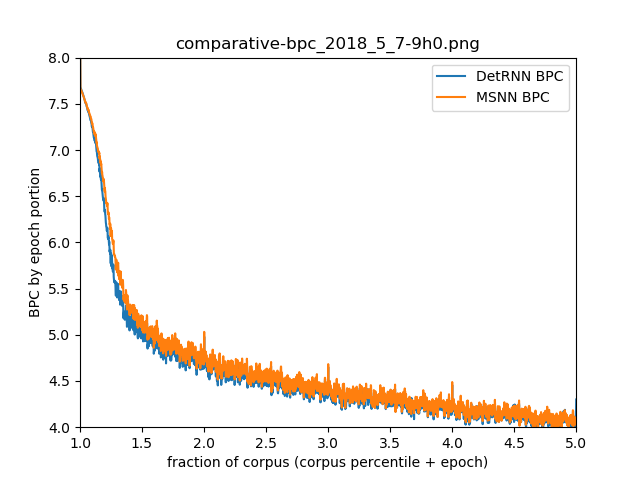
\includegraphics{parts/appendix/reports-gmsnn/docs_esteban-latex/test_reports/comparative-bpc-det-msnn_2018_5_7-9h0.png}
\caption{Comparative BPC}
\end{figure}

\subsubsection{Plot}

\paragraph{BPC/fraction of corpus}

BPS per fraction of the corpus (an interval of 1 correspond a complete
corpus, or an epoch).

\begin{figure}[h]
\centering
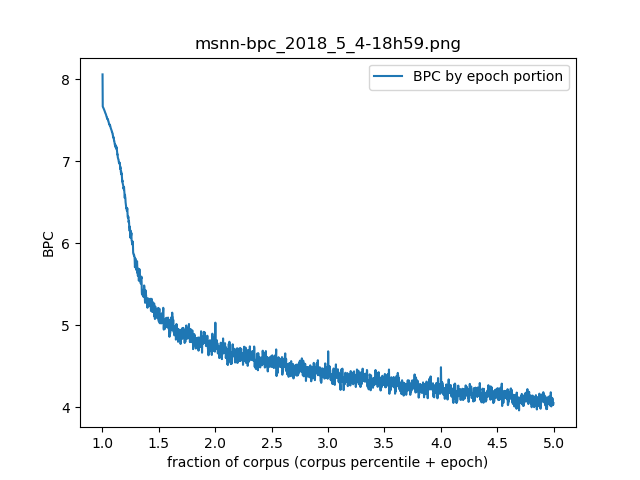
\includegraphics{parts/appendix/reports-gmsnn/docs_esteban-latex/test_reports/msnn-base/msnn-bpc_2018_5_4-18h59.png}
\caption{BPC}
\end{figure}

\paragraph{ValBPC/epoch}

Mean BPC over the epoch, at the end of each epoch.

\begin{figure}[h]
\centering
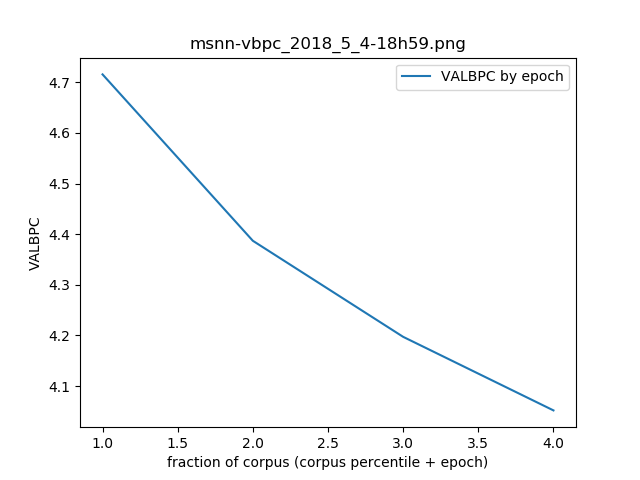
\includegraphics{parts/appendix/reports-gmsnn/docs_esteban-latex/test_reports/msnn-base/msnn-vbpc_2018_5_4-18h59.png}
\caption{ValBPC}
\end{figure}

\paragraph{Loss}

Loss per fraction of the corpus (an interval of 1 correspond a complete
corpus, or an epoch).

\begin{figure}[h]
\centering
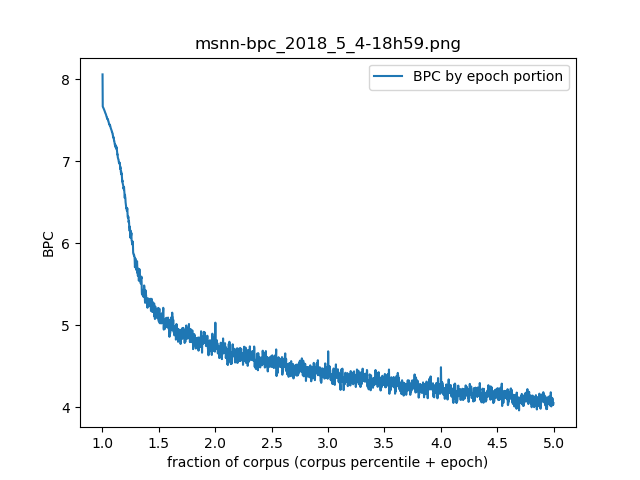
\includegraphics{parts/appendix/reports-gmsnn/docs_esteban-latex/test_reports/msnn-base/msnn-bpc_2018_5_4-18h59.png}
\caption{Loss}
\end{figure}

\subsubsection{Logs}

Reduced log is available at \href{msnn-base/msnn_2018_5_4-14h43.log}{msnn-base/msnn\_2018\_5\_4-14h43.log}.

\subsection{Potential ameliorations \& next steps}

A necessary amelioration is to add a way to track the number of layers.

As of now, the upper hidden layers participates in the output only when
updated. It is necessary to make them participate at every step.

The test process is not well defined: what to do when the eval batch is
dicontinuted from the training batch ? what if it is in the same corpus,
but not directly adjacent ? A possible yet hazardous solution would be
to evaluate a ``distance'' between the training and evaluation batches,
and reset the hidden states depending on that distance (a higher
distance would reset a higher number of layers).

Lastly, as the number of values to remember is increasing (bpc, loss,
layer number, \ldots{}) it would be interesting to improve the .plotdata
system.

Next step is to test the recurrently defined growing model.
